% IEEE TCAD submission format: two-column IEEE journal, 10 pt, US letter.
\documentclass[10pt,journal,letterpaper]{IEEEtran}
\usepackage{amsmath,amsfonts}
\usepackage{algorithmic}
\usepackage{algorithm}
\usepackage{array}
\usepackage[caption=false,font=footnotesize]{subfig}
\usepackage{textcomp}
\usepackage{stfloats}
\usepackage{url}
\usepackage{verbatim}
\usepackage{graphicx}
\usepackage{cite}
\usepackage{booktabs}
\usepackage{tabularx}
\usepackage{makecell}
\usepackage{xspace}
\usepackage{xcolor}
\newcommand{\sysname}{CircuitModelPilot\xspace}

\begin{document}

\title{CircuitModelPilot: An Agentic Framework for Automated Circuit Modeling across AI4EDA Tasks}

\author{Yongxun Liu, Bin Sun, Jianan Mu, Cheng Liu, and Huawei Li%
\thanks{Yongxun Liu is with the Hangzhou Institute for Advanced Study, University of Chinese Academy of Sciences, Hangzhou, China, and the University of Chinese Academy of Sciences, Beijing, China. He is also a research intern with the Institute of Computing Technology, Chinese Academy of Sciences, Beijing, China.}%
\thanks{Bin Sun, Jianan Mu, and Huawei Li are with the Institute of Computing Technology, Chinese Academy of Sciences, Beijing, China, and the University of Chinese Academy of Sciences, Beijing, China.}%
\thanks{Cheng Liu is with North China Electric Power University, China. \textit{Corresponding author: Cheng Liu.}}}



\markboth{IEEE Transactions on Computer-Aided Design of Integrated Circuits and Systems}%
{Liu \MakeLowercase{\textit{et al.}}: CircuitModelPilot: Automated Circuit Modeling across AI4EDA Tasks}


\maketitle




\section{Abstract}
\label{Abstract}

\begin{abstract}

Effective GNN predictors for electronic design automation (EDA) often require more than choosing a strong neural backbone: their learning formulation must be grounded in how the target EDA analysis operates. Automating such design therefore requires exploring task-level modeling hypotheses beyond the fixed search spaces of conventional GNN-NAS. While LLM agents provide a natural mechanism for such open-ended exploration, directly using them for EDA GNN research faces two fundamental challenges. First, a \textit{hypothesis-grounding gap} causes agents to favor generic architecture or training tweaks over hypotheses rooted in EDA objects, dependencies, and analysis semantics. Second, \textit{unreliable long-horizon execution} makes iterative hypothesis formulation, implementation, experimentation, and refinement vulnerable to context drift, uncontrolled code changes, and protocol violations.
We present \textbf{\sysname}, a hypothesis-driven auto-research harness for EDA-native GNN exploration. To address the grounding challenge, \sysname structures candidate hypotheses through \textit{semantic co-design}, organizing them across representation, computation, and learning signal so that each candidate corresponds to an explicit EDA modeling rationale. To address the execution challenge, \sysname organizes exploration as a \textit{hypothesis tree}, where each node represents a hypothesis-backed design state and each edge represents a controlled refinement. A scoped experimental protocol binds each hypothesis to its implementation scope, training configuration, evaluation result, and lineage, enabling systematic branching, replay, comparison, and evidence attribution. Experiments on HLS resource prediction, netlist-level timing prediction, and RTL-to-netlist timing prediction show that \sysname discovers accurate and reproducible EDA-native GNN designs beyond conventional GNN-NAS spaces.


\end{abstract}



\begin{IEEEkeywords}
Automated circuit modeling, electronic design automation (EDA), graph neural networks (GNNs), large language model (LLM) agents, model design search.
\end{IEEEkeywords}

\section{Introduction}
\label{introduction}

% 大背景
% GNN-based predictors have become an important class of learning-based surrogates for AI-assisted EDA, where many prediction tasks are defined over graph-structured design artifacts. They have been widely explored for resource estimation, timing prediction, congestion analysis, and design-space exploration, providing fast approximations to expensive EDA tools in modern design flows.

% % 观察到的现象，和现象解释
% Despite this promise, deploying GNN predictors across EDA tasks is not a plug-and-play process. Strong EDA GNN predictors are often not determined by the choice of a generic backbone alone. Their effectiveness often depends on whether the graph-learning problem is formulated to reflect the reasoning structure of the target EDA analysis. Timing prediction provides a representative example: an effective predictor must expose timing-relevant objects, propagate delay-related information along circuit dependencies, and use meaningful intermediate timing quantities to guide learning beyond the final label.
% {\color{blue}[Fig1]}

  
% This difficulty is intrinsic to EDA prediction. Unlike ordinary graph labels, EDA labels are tool-induced properties computed over realized design states, for example after synthesis, implementation, or scheduling. Rather than directly annotating isolated graph nodes or edges, these labels summarize task-specific analyses over hidden design states and constraints. When a predictor is given only a generic graph and the final label, these task semantics remain implicit, forcing the model to recover them statistically from data. This makes EDA prediction an under-specified and data-inefficient inverse problem, where the model may exploit superficial label correlations instead of learning the analysis structure that gives rise to the target property. The core issue is thus not merely whether the GNN backbone is expressive enough, but whether the learning formulation exposes the task objects, dependencies, and intermediate quantities needed to make the target EDA analysis learnable.

% % 现象蕴含出的方法论
% This observation shifts the design target from choosing a better GNN backbone to formulating a better EDA graph-learning problem. We call this process \textit{semantic co-design}: graph representation, GNN computation, and learning signal are designed as mutually consistent realizations of the same task-level hypothesis about how an EDA property is produced. 
% % In this view, the key question is not only which neural primitive to use, but also what design objects should be exposed, how task-relevant information should propagate, and which intermediate quantities should shape the learned representationl
% {\color{blue}[Fig2]}

% \begin{figure}[tb!]
%   \centering

%   \subfloat[]{%
%     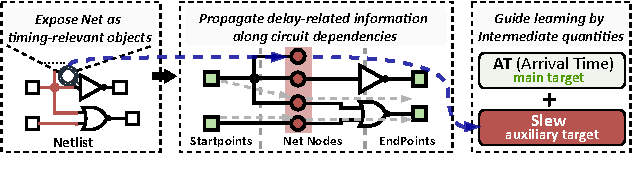
\includegraphics[width=1\linewidth]{figs/Q-1.pdf}
%     \label{fig:problem-1}
%   }\\[-0.1em]

%   \subfloat[]{%
%     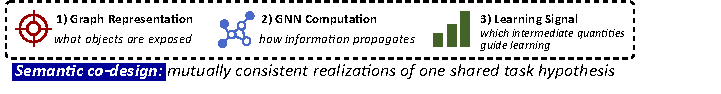
\includegraphics[width=1\linewidth]{figs/Q-2.pdf}
%     \label{fig:problem-2}
%   }\\[-0.8em]   % 重点：减小 b 和 c/d 之间的距离

%   \subfloat[]{%
%     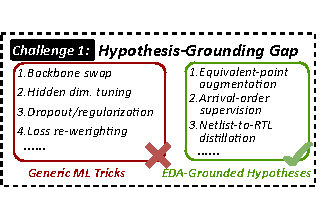
\includegraphics[width=0.49\linewidth]{figs/Q-3.pdf}
%     \label{fig:problem-3}
%   }
%   \hfill
%   \subfloat[]{%
%     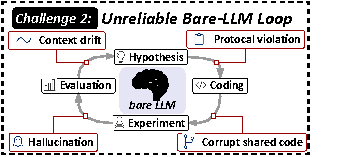
\includegraphics[width=0.48\linewidth]{figs/Q-4.pdf}
%     \label{fig:problem-4}
%   }

%   \caption{\textbf{TODO}}
%   \label{fig:problem}
% \end{figure}



% % 挑战部分
% Realizing semantic co-design requires searching beyond a fixed set of neural primitives. Since task-level modeling hypotheses are often easier to express in language than to enumerate as NAS operators, LLM agents offer a promising search mechanism: they can reason about the EDA task, propose meaningful hypotheses, and translate them into feature engineering, model or training improvement.

% However, two challenges limit their direct use. First, a \textit{hypothesis-grounding gap} arises because general-purpose agents tend to generate generic ML tricks, such as backbone replacement or hyperparameter tuning, rather than EDA-grounded hypotheses derived from design objects, tool semantics, structural dependencies, or intermediate analysis quantities. Second, an \textit{unreliable bare-LLM loop} makes long-horizon auto-research difficult: as the agent repeatedly performs hypothesis formulation, coding, experimentation, and evaluation, lengthy EDA tool reports and accumulating experimental states can cause context drift, hallucination, protocol violations, and unintended edits to shared code. Consequently, even runnable candidates may lack clear domain rationale, reliable comparison, and attributable evidence.
% {\color{red}[E5: hypothesis-grounding and bare-LLM reliability study.]}
% {\color{blue}[Fig3\&4]}

% % 方法 TODO
% To address these challenges, we propose \textbf{SCOPE}, a protocol-grounded agentic framework for EDA-native GNN design. SCOPE uses LLM agents to explore semantic co-design hypotheses beyond fixed NAS primitives. To preserve \textit{hypothesis grounding}, SCOPE organizes each candidate around three semantic levels---representation, computation, and learning signal---and requires the candidate to correspond to an explicit EDA modeling rationale. To preserve \textit{evidence attribution}, SCOPE evaluates each candidate through a scoped task interface and records it as a design trace that binds the hypothesis, implementation scope, training configuration, validation result, and parent-child relation. This allows SCOPE to keep the search space open enough for task-level modeling hypotheses, while making each discovered improvement comparable, replayable, and attributable.

% % Evaluation
% We evaluate SCOPE on representative AI EDA prediction tasks, including HLS resource prediction, netlist-level timing prediction, and RTL-to-netlist timing prediction. The evaluation examines whether SCOPE discovers EDA-native designs beyond conventional GNN-NAS spaces, whether its protocol improves attribution and reproducibility over naive LLM exploration, and whether the discovered predictors improve accuracy over human baselines and automated search baselines. {\color{red}[E6: final benchmark results to be inserted.]}

% The contributions are summarized as follows:
% \begin{itemize}
% \item \textbf{Observation.} We characterize effective EDA GNN design as \textit{semantic co-design}, where representation, computation, and learning signal are jointly aligned with the reasoning structure of the target EDA analysis. We support this characterization through literature taxonomy and controlled pre-experiments.

% \item \textbf{Method.} We introduce \textbf{SCOPE}, a protocol-grounded agentic framework that uses LLM agents to search EDA-native design hypotheses, while enforcing hypothesis grounding through semantic-level organization and evidence attribution through scoped interfaces and design traces.

% \item \textbf{Evaluation.} We evaluate SCOPE across representative EDA prediction tasks and compare it with human baselines, conventional GNN-NAS, and naive LLM-based exploration. {\color{red}[Experimental results to be inserted.]}

% \end{itemize}


\IEEEPARstart{G}{NN-based} predictors have become an important class of learning-based surrogates for AI-assisted electronic design automation (EDA), where many prediction tasks are defined over graph-structured design artifacts. They have been widely explored for resource estimation, timing prediction, congestion analysis, and design-space exploration, providing fast approximations to expensive EDA tools in modern design flows.
However, developing an effective GNN predictor for an EDA task is rarely a matter of selecting a stronger neural backbone alone. EDA prediction targets are produced by structured analysis procedures---such as synthesis, scheduling, static timing analysis, or physical implementation---and an effective learning formulation often needs to reflect the task-specific semantics underlying these procedures. In practice, many successful EDA GNNs therefore rely on manually designed choices about what design information should be exposed to the model, how task-relevant information should be propagated, and what intermediate semantics should guide learning. We refer to the coordinated design of these choices as \textit{semantic co-design}.

The automation of GNN design has evolved through two existing paradigms, yet both remain insufficient for EDA-native model research. \textbf{First, conventional GNN-NAS and AutoML} automate model selection within expert-defined search spaces, such as neural operators, aggregation functions, depth, normalization, and training hyperparameters. Their automation is therefore limited to choices that have already been enumerated. \textbf{Second, recent LLM-based research agents} remove this restriction by directly proposing and implementing open-ended code modifications, substantially expanding the space of possible designs. However, unrestricted exploration alone is not enough: as the search space becomes more open, useful research increasingly depends on \emph{narrowing} exploration toward hypotheses that are meaningful for the target domain. Motivated by this limitation, we propose a third paradigm for EDA GNN automation: \textbf{hypothesis-driven auto-research}, where the fundamental unit of exploration is neither a predefined architecture choice nor an arbitrary code patch, but an explicit EDA modeling hypothesis. The key is to retain the open-ended generation capability of LLM agents while progressively narrowing it into grounded and testable research directions.

Realizing hypothesis-driven AutoResearch introduces two challenges. \textbf{(1) Hypothesis-grounding gap:} open-ended agents often fall back to generic ML modifications, such as backbone replacement, hidden-dimension tuning, regularization, or loss reweighting, rather than hypotheses derived from EDA-specific objects, dependencies, and analysis semantics. \textbf{(2) Unreliable long-horizon execution:} even with a meaningful initial hypothesis, repeated hypothesis formulation, coding, experimentation, and evaluation can lead to context drift, uncontrolled code changes, protocol violations, and ambiguous attribution of performance improvements.

To address the first challenge, we use \textit{semantic co-design} to narrow open-ended hypothesis generation into three EDA-grounded levels: \textbf{representation}, which determines what task-relevant objects and dependencies are exposed; \textbf{computation}, which determines how task-relevant information propagates; and \textbf{learning signal}, which determines what intermediate EDA semantics guide learning. These levels do not enumerate concrete model candidates. Instead, they define where meaningful hypotheses should be sought, allowing the agent to generate previously unspecified designs while remaining grounded in the reasoning structure of the target EDA analysis.

To address the second challenge, we organize agent execution as a \textit{hypothesis tree}. Each node represents a hypothesis-backed research state, and each edge represents a controlled refinement of its parent. Rather than evolving a single long and entangled research trajectory, the agent can explicitly branch from promising states, compare alternative refinements, revisit earlier hypotheses, and prune ineffective directions. A scoped experimental protocol further binds each hypothesis to its implementation scope, training configuration, evaluation result, and lineage, making the resulting exploration replayable, comparable, and attributable.

Based on these mechanisms, we present \textbf{\sysname}, a hypothesis-driven AutoResearch harness for EDA-native GNN exploration. \sysname combines semantic narrowing with hypothesis-tree execution: semantic co-design determines \emph{what kinds of hypotheses are meaningful to explore}, while the hypothesis tree and scoped protocol determine \emph{how those hypotheses are reliably executed and refined}. Together, they preserve the flexibility of LLM-based exploration without reducing automated research to either a fixed NAS space or unconstrained trial-and-error.

% Evaluation
We evaluate \sysname on representative AI-for-EDA prediction tasks, including HLS resource prediction, netlist-level timing prediction, and RTL-to-netlist timing prediction. Our evaluation examines whether \sysname discovers EDA-native GNN designs beyond conventional GNN-NAS spaces, whether semantic grounding and hypothesis-tree execution improve research reliability over naive LLM exploration, and whether the discovered predictors outperform human-designed and automated-search baselines. {\color{red}[E6: final benchmark results to be inserted.]}

The contributions are summarized as follows:
\begin{itemize}
\item \textbf{Hypothesis-driven AutoResearch.} We introduce a new automation paradigm for EDA-native GNN research that moves beyond predefined architecture search and unconstrained LLM code exploration. The key principle is to preserve open-ended generation while narrowing it toward explicit, testable EDA modeling hypotheses.

```
\item \textbf{Semantic hypothesis grounding.} We use representation, computation, and learning signal as three semantic levels for narrowing open-ended exploration toward EDA-grounded hypotheses, without requiring experts to enumerate concrete candidate designs in advance.

\item \textbf{Hypothesis-tree execution.} We organize long-horizon agent exploration as a hypothesis tree with scoped experimental protocols, enabling controlled refinement, branching, replay, comparison, and evidence attribution across research trajectories.

\item \textbf{Evaluation.} We evaluate \sysname across representative EDA prediction tasks against human-designed baselines, conventional GNN-NAS, and naive LLM-based exploration. {\color{red}[Experimental results to be inserted.]}
```

\end{itemize}




\section{Related Work}
\label{background}

AI-for-EDA (AI4EDA) uses learned models to support circuit analysis and optimization, including power, performance, and area estimation, timing prediction, and routability assessment. Predictors trained on circuit descriptions and tool-generated measurements can provide early feedback before expensive downstream analysis. The development of these predictors has progressively expanded from fitting models to engineered features, through learning circuit representations, to automating model design and experimentation. These approaches remain complementary; the progression highlights how the scope of automation has grown and which modeling decisions still require human expertise.

\subsection{Feature Engineering and Traditional Machine Learning}
\label{sec:feature_based_modeling}

Early learning-based circuit models typically started from a clearly specified prediction problem and a set of features selected by domain experts. Designers summarized relevant properties, such as switching activity, resource counts, or timing statistics, and fitted statistical or machine-learning models to the resulting feature vectors. Regression-based RTL power modeling by Bogliolo et al.~\cite{bogliolo2000regression}, for example, used linear regression and nonparametric extensions to relate power dissipation to input and output activity. For HLS, Dai et al.~\cite{dai2018fast} extracted features from synthesis reports and compared predictive models for estimating post-implementation quality of results.

These methods established the value of inexpensive learned approximations to EDA analyses. Their effectiveness nevertheless depended strongly on the information retained by the feature extractor. Once a circuit had been reduced to a fixed feature vector, the learner could exploit relationships among those features but could not recover omitted structural dependencies. Improving the predictor therefore often required an engineer to reconsider the feature set using knowledge of both the target EDA analysis and the learning method.

\subsection{Deep Learning for Circuit Prediction}
\label{sec:deep_circuit_modeling}

Deep learning shifted part of this effort from manually specifying feature interactions to learning them through neural architectures. Fully connected networks can learn nonlinear mappings from circuit descriptors, while convolutional neural networks (CNNs) can exploit spatial regularity in layout-derived inputs. RouteNet~\cite{xie2018routenet} illustrates the latter approach: it represents placement information as image-like inputs and applies CNNs to predict overall routability and design-rule-checking hotspots. This formulation connects the spatial structure of the prediction problem with an architecture suited to processing it.

Learned representations expanded the range of relationships that a predictor could capture, but model development still required substantial manual choices about input encoding, network architecture, training data, and optimization. A layout image is useful for spatial effects, whereas circuit connectivity need not follow proximity on that image. Likewise, a fully connected network operating on aggregate descriptors does not explicitly expose relationships between individual circuit elements. These limitations motivated models that process circuit structure more directly, alongside continued use of CNNs for spatial prediction tasks.

\subsection{Graph Neural Networks and Circuit-Specific Model Design}
\label{sec:semantic_codesign}

GNNs provide a natural representation for irregular circuit structures by treating operations, gates, pins, or other design objects as nodes and their dependencies as edges~\cite{lopera2021survey}. Compared with flattening a design into a fixed vector or rasterizing it onto a grid, graph-based modeling can explicitly retain connectivity and propagate information along task-relevant relations. Representative work spans HLS program graphs, netlist timing graphs, and logic representations, showing that the graph abstraction and learning procedure must be adapted to the property being predicted.

The existing literature illustrates three coupled dimensions of this adaptation. \emph{Representation (L1)} determines which circuit objects, relations, and features are visible to the model. GNN-DSE~\cite{sohrabizadeh2022automated} and Balor~\cite{murphy2024balor} develop graph-based HLS predictors, with Balor combining custom source-code graphs and hierarchical GNNs. \emph{Computation (L2)} determines how information is propagated and combined. PowerGear~\cite{lin2022powergear} uses a heterogeneous edge-centric GNN for power estimation, while the timing-engine-inspired model of Guo et al.~\cite{guo2022timing} structures prediction around timing propagation. \emph{Learning signal (L3)} determines the objectives and supervision used to train the representation. Guo et al. use local edge-delay prediction as auxiliary supervision, and DeepGate2~\cite{shi2023deepgate2} uses differences between sampled gates' truth tables to teach circuit functionality. These dimensions overlap: an effective improvement may require coordinated changes to the graph, the computation, and the training objective.

Thus, graph structure makes circuit information more accessible to a learner, but it also introduces additional modeling decisions. Engineers must construct appropriate graphs and datasets, choose node and edge attributes, design propagation and readout mechanisms, and select training objectives that reflect the target analysis. Data generation and labeling further depend on EDA tools and design constraints. Successful model development consequently draws on both machine-learning expertise and an understanding of circuits and EDA, motivating automation beyond parameter fitting alone.

\subsection{Neural Architecture Search and Automated Model Selection}
\label{sec:automated_gnn_design}

Neural architecture search (NAS) reduces the effort of manually selecting neural components by optimizing their combinations within a specified design space. Chang et al.~\cite{chang2020automatic} apply NAS to routability predictor development, providing an EDA-specific example of automated architecture construction. For graph learning, GraphNAS~\cite{gao2019graphnas} and Auto-GNN~\cite{zhou2022auto} use reinforcement-learning-based search to select GNN architectures, while the systematic design-space study of You et al.~\cite{you2020design} examines architectural and training choices across graph-learning tasks. These efforts make it easier to obtain competitive configurations without manually testing each candidate.

The remaining boundary is the design space itself. Available operators, connectivity patterns, and tunable settings must be represented in the search procedure, which evaluates candidates against a prescribed performance objective. The amount of manual architecture exploration is reduced, but experts still define the circuit representation, permissible transformations, and often the learning objective. If validation errors reveal a missing circuit relation or an unsuitable propagation rule, a fixed-space search can address that limitation only when the relevant change is already expressible. Automating this further step requires interpreting the model's behavior and creating new modeling strategies, rather than only selecting among encoded alternatives.

\subsection{LLM Agents and Autonomous Circuit Modeling}
\label{sec:llm_agents}

LLM-based research systems extend automation to proposing changes, editing code, running experiments, and interpreting results. The AI Scientist~\cite{lu2024aiscientist} connects idea generation with implementation, experimentation, and scientific reporting. AutoResearch~\cite{karpathy2026autoresearch} focuses on iterative modification and evaluation of language-model training code. Arbor~\cite{jin2026arbor} organizes autonomous research around a persistent tree of proposals, artifacts, evidence, and accumulated insights. These systems demonstrate mechanisms for carrying experimental findings into subsequent attempts and reducing repeated human intervention in the development loop.

Circuit modeling benefits from these capabilities, but useful feedback must also reflect the EDA problem being learned. An aggregate validation score establishes whether a predictor improves under the selected metric; additional circuit-specific analysis can help explain where it fails and what to change. For example, timing errors can be examined by path depth or cell type to investigate deficiencies in information propagation, while resource-prediction errors can be related to operation types or synthesis transformations. Such diagnostics turn circuit knowledge into evidence that can guide changes to representations, architectures, or training objectives. They complement general observations about convergence, capacity, and optimization with information about the physical or logical relationships the model is intended to capture.

CircuitModelPilot builds on the emerging autonomous-research workflow with this circuit-modeling focus. It uses task descriptions, circuit knowledge, and experimental feedback to analyze the current model, propose a revised modeling strategy, generate its implementation, and test the result. A model-design search tree retains alternative candidates and their outcomes so that later iterations can extend useful directions and reconsider unsuccessful ones. Relative to fixed-space NAS, the framework can introduce implementations that were not enumerated beforehand; relative to general research or training agents, its emphasis is on using EDA-specific evidence to make modeling revisions more targeted. The goal is to reduce the combined AI and EDA engineering effort needed to develop task-specific predictors and advance toward autonomous circuit modeling.

\section{Framework}
\label{framework}

CircuitModelPilot automates the iterative development of circuit predictors, from analyzing an existing model to implementing and evaluating a revised design. Given an AI4EDA task and an initial predictor, the framework uses LLM agents to inspect model behavior, identify potential deficiencies in the circuit-modeling formulation, and turn proposed improvements into executable candidates. Candidate designs are organized in a search tree so that the framework can explore alternatives, revisit earlier models, and use both positive and negative experimental feedback. The same workflow supports changes to circuit representations, neural computation, and learning objectives, together with training and hyperparameter optimization. This section formalizes the modeling problem, presents the overall architecture, and describes the components that implement this iterative search.

\subsection{Problem Formulation}
\label{sec:problem_formulation}

\subsubsection{Circuit Modeling as a Design Problem}

Let $\mathcal{D}_{\mathrm{tr}}$ and $\mathcal{D}_{\mathrm{val}}$ denote the training and validation data for an EDA prediction task. A modeling formulation is
\begin{equation}
    \mathcal{C}=(\phi,\psi,\ell),
    \label{eq:codesign_tuple}
\end{equation}
where $\phi$ constructs the circuit representation and its features, $\psi$ specifies the neural architecture and computation, and $\ell$ specifies the training objective, including any auxiliary supervision. These correspond to the representation, computation, and learning-signal dimensions discussed in Section~\ref{sec:semantic_codesign}. Training a candidate with configuration $\lambda$ produces parameters
\begin{equation}
    \theta=\operatorname{Train}(\mathcal{C},\lambda;
    \mathcal{D}_{\mathrm{tr}}),
    \label{eq:candidate_training}
\end{equation}
and a predictor $f_{\mathcal{C},\theta}(d)=\psi_{\theta}(\phi(d))$. We write its validation utility as
\begin{equation}
    q=Q(f_{\mathcal{C},\theta};\mathcal{D}_{\mathrm{val}}),
    \label{eq:validation_utility}
\end{equation}
with the metric direction normalized so that larger $q$ is better. For example, an error metric can be negated. The prediction target, label meaning, and validation metric remain fixed even when a candidate changes the objective used for gradient-based training. Thus, redesigning $\ell$ does not redefine what counts as a better predictor.

\subsubsection{Distinction from Fixed-Space NAS}

A conventional architecture-search formulation can be expressed as
\begin{equation}
    (a^\star,\lambda^\star)
    =\operatorname*{arg\,max}_{a\in\mathcal{A}_{\mathrm{NAS}},\,
    \lambda\in\Lambda} q(a,\lambda),
    \label{eq:fixed_nas}
\end{equation}
where $\mathcal{A}_{\mathrm{NAS}}$ and $\Lambda$ encode available architecture and training choices. Typically, circuit representation and supervision are supplied by the task designer; even when they are searchable, their alternatives must be expressible in the predefined space. Feedback guides selection among these encoded choices.

CircuitModelPilot instead constructs new formulations during search. At iteration $t$, it selects a parent $p$ and generates a modeling proposal $P_{t+1}$ using the task context $\kappa$, circuit knowledge $\mathcal{K}$, the current search tree $\mathcal{T}_t$, and the parent's experimental evidence $E_p$:
\begin{equation}
\begin{aligned}
 P_{t+1}&=\pi_{\mathrm{LLM}}
 (\kappa,\mathcal{K},\mathcal{T}_t,E_p),\\
 \mathcal{C}_{t+1}&=\operatorname{Implement}
 (\mathcal{C}_p,P_{t+1}).
\end{aligned}
\label{eq:adaptive_modeling}
\end{equation}
The proposal may introduce a graph transformation, a propagation mechanism, or a training objective whose implementation was not listed initially. The task interface and editable modules constrain these changes, but do not enumerate all resulting models. The LLM uses both performance and diagnostic evidence to decide what to construct, while the fixed validation utility still determines how candidates are compared.

Under a total search budget $B$, the output is selected from the successfully evaluated candidates $\mathcal{V}_{\mathrm{ok}}$:
\begin{equation}
\begin{aligned}
 i^\star&=\operatorname*{arg\,max}_{i\in\mathcal{V}_{\mathrm{ok}}}q_i,\\
 \sum_{r\in\mathcal{R}}c_r&\leq B,
\end{aligned}
\label{eq:semantic_search}
\end{equation}
where $\mathcal{R}$ includes all attempted runs and $c_r$ is their cost under the declared budget measure. This is a budgeted search over generated candidates, without a claim of global optimality. Training and tuning costs, including unsuccessful attempts, must be included consistently in comparisons with automated baselines.

\subsection{Overall Architecture}
\label{sec:framework_overview}

Figure~\ref{fig:framework} shows the CircuitModelPilot workflow. A task interface supplies circuit knowledge, data access, the initial model, and training and evaluation entry points. The search controller selects a parent from the model-design tree. A modeling agent diagnoses its limitations and proposes a revision; a candidate builder implements the revision and checks that the code matches the proposal. The execution component trains the candidate, optionally tunes its hyperparameters, and collects validation results. A result analyst interprets the evidence and recommends how exploration should proceed. The candidate and its analysis are then added to the tree, closing the feedback loop.

\begin{figure*}[t]
    \centering
    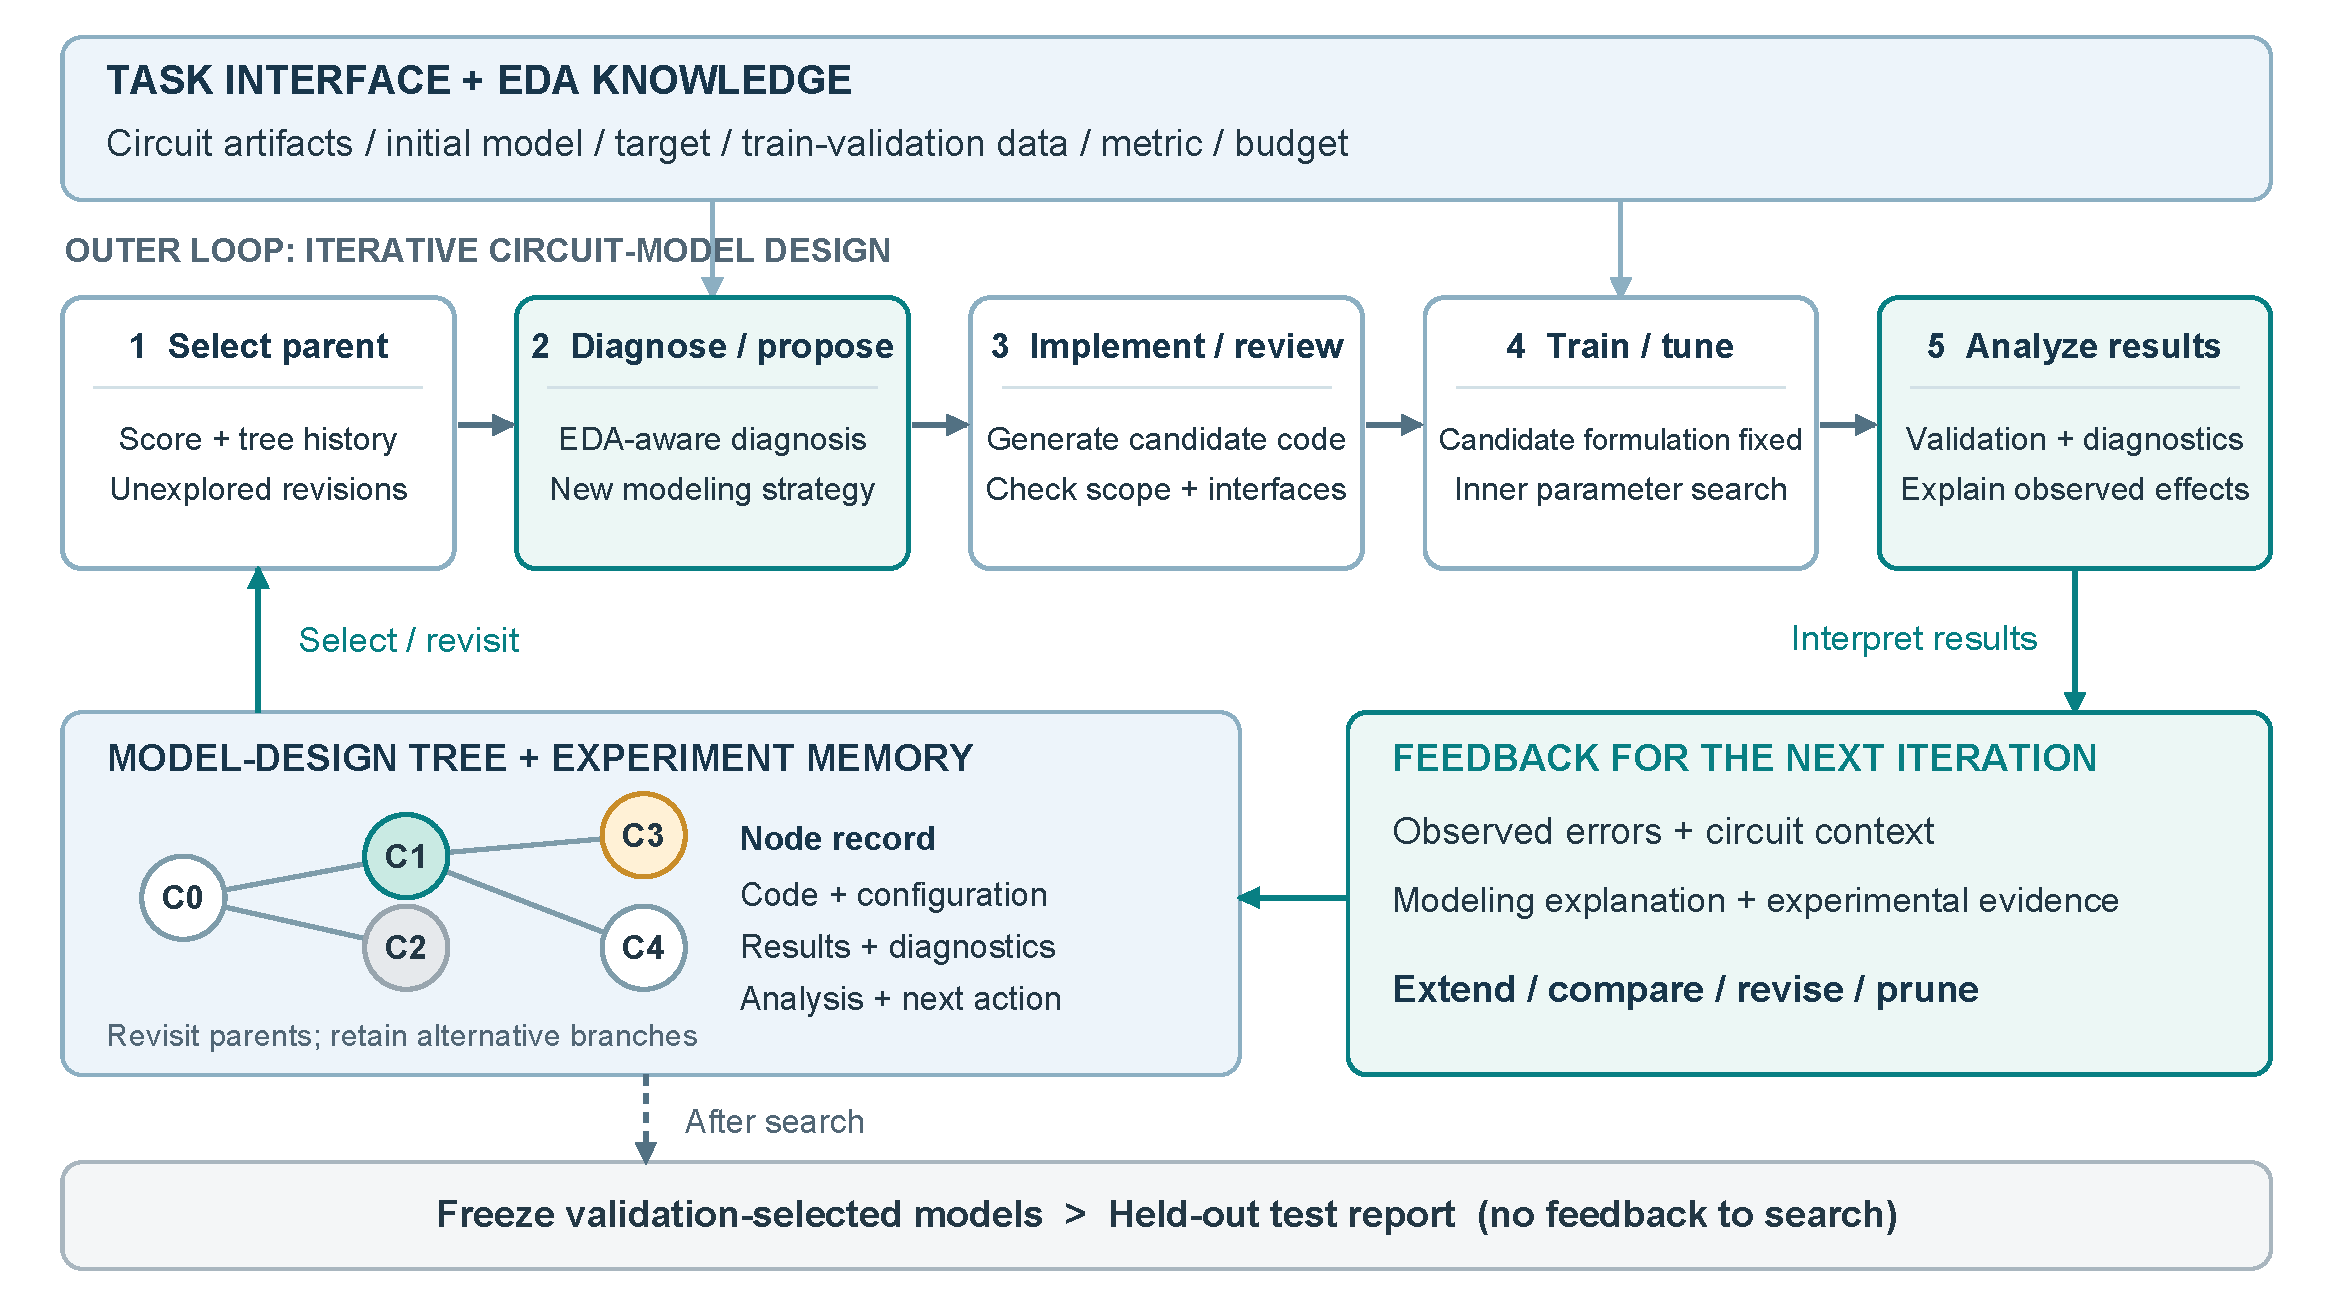
\includegraphics[width=\textwidth]{figs/CircuitModelPilot-framework.pdf}
    \caption{Overall architecture of CircuitModelPilot. The LLM-guided outer loop constructs and evaluates new circuit-modeling strategies, while the inner training and tuning stage optimizes each candidate. Circuit knowledge and validation diagnostics guide subsequent revisions through a persistent model-design tree. Held-out test evaluation occurs only after model selection and has no feedback path into search.}
    \label{fig:framework}
\end{figure*}

The components have distinct responsibilities: the modeling agent decides what to change, the builder realizes that change, the executor measures its effect, and the analyst determines what the evidence supports. They are roles in the workflow and need not correspond to different LLM families. Shared experiment records connect them across iterations and allow the search controller to return to an earlier candidate without reconstructing its state from a conversation history.

\subsection{Task Interface and EDA Knowledge}
\label{sec:task_interface}

Each task adapter defines the prediction target, available circuit artifacts, input and output contracts, initial predictor, permitted code modules, and training and validation procedures. It also fixes the data partition, metric definition, and budget policy in the task context $\kappa$. Candidate-generated preprocessing operates within this interface so that a representation change remains compatible with the task and does not alter the evaluation samples or their labels.

The adapter provides the domain information needed to interpret model behavior: circuit object and relation types, relevant analysis rules, feature meanings, and available diagnostic quantities. For netlist timing, this may include cell types, timing arcs, and path dependencies. For HLS prediction, it may include operations, data dependencies, and synthesis-related attributes. CircuitModelPilot uses this information together with model code and experimental observations to reason about what the current predictor captures and what it may omit. The framework therefore reuses a common agent workflow across tasks while retaining task-specific representations and diagnostics.

Domain knowledge also determines which questions can be answered by the available evidence. If a task exposes only aggregate error, the agent may request an additional validation diagnostic before proposing a structural change. It should not infer a particular circuit-level failure from the aggregate score alone. All diagnostics used for search are derived from the training or validation partition; the held-out test set remains outside the agent's working context.

\subsection{Model Diagnosis and Revision Proposals}
\label{sec:hypothesis_protocol}

For a selected parent, the modeling agent examines three sources of evidence: the current implementation, its validation and training behavior, and the history of related candidates. It relates observed errors to the task's circuit representation and analysis structure. For example, errors concentrated on deep timing paths may suggest insufficient propagation of delay information; errors concentrated on a cell category may suggest that distinct cell behavior is being aggregated too uniformly. These are possible explanations to investigate, rather than conclusions implied by an error pattern.

The agent converts its analysis into a concise modeling proposal containing the observed limitation, the proposed change, its implementation scope, and the diagnostic effect expected if the change is useful. The proposal is stored in the existing hypothesis-card artifact, but its purpose is practical: to connect a modeling decision to code and an experiment. A proposal can involve coordinated changes, such as adding a graph relation and its corresponding update rule, while unrelated changes are assigned to separate candidates so their effects remain interpretable.

The available revision dimensions are those in $\mathcal{C}$. Representation changes can expose additional circuit objects, features, or relations. Computation changes can revise message passing, aggregation, update order, or prediction heads. Learning changes can revise loss transformations or auxiliary supervision. The agent selects among these dimensions according to the observed limitation; it does not have to modify every dimension in each iteration. Prior failed attempts constrain later proposals by recording which modifications were tested and under what conditions they were unsuccessful.

\subsection{Candidate Implementation, Training, and Tuning}
\label{sec:scoped_realization}

\subsubsection{Code Generation and Candidate Review}

The builder copies the selected parent's generated modules into a candidate workspace and implements the proposed revision there. The supported modules include graph transformations, model and convolution definitions, and task-approved training components. The parent implementation is retained so that alternative children can branch from the same starting point.

Before training, a separate Candidate Review checks whether the proposed modeling change is realized in the code and whether additional changes have been introduced. Runtime checks validate interfaces, editable scope, and the task context. A failed implementation is repaired within the same proposal or recorded as an unsuccessful attempt. A code error is not treated as evidence that the modeling idea itself is ineffective. The candidate record retains the proposal, source snapshot, parent-relative changes, and execution configuration.

\subsubsection{Training and Inner Parameter Search}

For a fixed formulation $\mathcal{C}_i$, the executor trains the model and selects checkpoints using validation evidence. When enabled by the task, a separate inner search selects a training configuration:
\begin{equation}
 \lambda_i^\star=\operatorname*{arg\,max}_{\lambda\in\Lambda_i}
 Q\big(f_{\mathcal{C}_i,\theta_i(\lambda)};
 \mathcal{D}_{\mathrm{val}}\big),
 \label{eq:param_search}
\end{equation}
where $\Lambda_i$ is the declared set of permitted hyperparameters and $\theta_i(\lambda)$ is obtained by training under that configuration. In practice, this denotes the best evaluated configuration within the allocated tuning budget. The existing execution workflow uses Optuna for this stage when parameter search is requested.

This separation distinguishes a change in modeling formulation from a change in its optimization settings. Both may improve prediction, but their contributions are recorded separately. The executor returns the validation score, permitted error breakdowns, training statistics, execution status, and cost. These observations support both candidate ranking and the next round of modeling analysis.

\subsection{Tree-Structured Model Search}
\label{sec:trace_guided_exploration}
\label{sec:design_trace}

\subsubsection{Tree State and Parent Selection}

The search state is a rooted tree $\mathcal{T}_t=(\mathcal{V}_t,\mathcal{E}_t)$ initialized with the baseline model. Each node stores a candidate record
\begin{equation}
 T_i=(p_i,\mathcal{C}_i,P_i,\lambda_i,E_i,A_i),
 \label{eq:design_trace}
\end{equation}
where $p_i$ identifies the parent, $P_i$ is the proposal, $E_i$ contains execution and validation evidence, and $A_i$ records the analysis and suggested next action. An edge $(p_i,i)$ represents the implemented revision. Nodes retain their artifacts and execution status even when a branch is no longer expanded.

Let $\mathcal{F}_t$ denote the set of evaluated candidates eligible for further development. It can include an earlier internal node, not only the most recent leaves. Parent selection is expressed as
\begin{equation}
 p_t=\pi_{\mathrm{select}}
 (\mathcal{F}_t,\mathcal{T}_t,\kappa,\mathcal{K}).
 \label{eq:parent_selection}
\end{equation}
The controller uses the LLM to weigh validation performance, remaining modeling limitations, evidence from previous children, and the remaining budget. It can refine a strong candidate or revisit an earlier node when another modeling direction remains plausible. The selected parent and the rationale for expanding it are recorded with the next proposal.

\subsubsection{Expansion, Comparison, and Pruning}

Expanding a node creates a child with one coherent modeling revision. Siblings provide alternative responses to the same parent limitation, while deeper descendants accumulate useful changes. An ablation is represented as another child that removes or alters a component to investigate its effect. Re-evaluations can be recorded as children with unchanged model code to distinguish repeatability evidence from a newly designed model.

After evaluation, the controller updates the eligible set using the result analysis. A promising child can remain active for refinement; a branch with repeated negative evidence can be marked inactive; an ambiguous result can trigger a focused diagnostic or another run within budget. Pruning changes future search allocation without deleting the candidate or its evidence. Returning to the root or another earlier node creates an alternative path through the same tree. These operations preserve useful work while preventing the search from being tied to one sequence of edits.

Algorithm~\ref{alg:hedge_loop} summarizes the process. Every attempted execution contributes to the search record and consumes budget according to the declared policy. The search stops when the budget is exhausted, no eligible direction remains, or the controller records an explicit stop decision. No monotonic improvement is assumed: failed candidates are part of the evidence used to choose later revisions.

\begin{algorithm}[t]
\caption{Iterative Circuit-Model Search}
\label{alg:hedge_loop}
\begin{algorithmic}[1]
\REQUIRE Task context $\kappa$, knowledge $\mathcal{K}$, initial model $\mathcal{C}_0$, budget $B$
\STATE Evaluate $\mathcal{C}_0$; initialize tree $\mathcal{T}$ and eligible set $\mathcal{F}$
\WHILE{budget remains and $\mathcal{F}\neq\emptyset$}
    \STATE Select parent $p$ using performance and recorded analysis
    \STATE Diagnose $\mathcal{C}_p$; propose a modeling revision $P_i$
    \STATE Implement and review candidate $\mathcal{C}_i$
    \IF{candidate passes review and runtime checks}
        \STATE Train and optionally tune within remaining budget
        \STATE Collect validation results and permitted diagnostics
        \STATE Analyze the outcome and recommend a next action
    \ELSE
        \STATE Record implementation failure and repair feedback
    \ENDIF
    \STATE Store child record in $\mathcal{T}$; account for consumed budget
    \STATE Update eligible parents $\mathcal{F}$ and search memory
    \IF{controller records a stop decision}
        \STATE \textbf{break}
    \ENDIF
\ENDWHILE
\STATE Freeze validation-selected candidates for final reporting
\end{algorithmic}
\end{algorithm}

\subsection{Feedback-Driven Iteration and Final Selection}
\label{sec:feedback_iteration}

The result analyst converts each completed experiment into feedback for the next design decision. It first checks whether the intended change was executed and the comparison is valid. For a successfully evaluated child, its utility difference from the parent is
\begin{equation}
    \Delta q_i=q_i-q_{p_i}.
    \label{eq:parent_improvement}
\end{equation}
The analyst interprets this difference alongside circuit-specific error breakdowns, learning curves, and the parent-relative code changes. It separates an observed performance change from an explanation of that change: a better aggregate score alone does not establish that the proposed mechanism resolved the diagnosed limitation.

Feedback addresses three questions: what improved or degraded, what the evidence suggests about the current modeling formulation, and which experiment should follow. If the expected diagnostic behavior improves with the score, the next iteration can extend the candidate or test the contribution of its components. If an intended effect is absent, the agent can revise the explanation and return to an earlier model. If the outcome is unstable or the diagnostic evidence is insufficient, the next action can be a repeat or a narrower test. The existing analysis records express these outcomes as supported, refuted, or inconclusive, with actions such as extend, ablate, prune, restart, or stop.

For example, a timing candidate that changes message propagation can be evaluated both on aggregate validation error and on errors grouped by path depth. Improvement concentrated on deeper paths would provide more specific feedback than the aggregate score alone. If errors instead persist for particular cell types, the next proposal may investigate cell-dependent transformations. This illustrates how the framework uses circuit knowledge to move from an observed limitation to a modeling change, then uses the experiment to refine the next question.

Each analysis is saved with the corresponding node so that subsequent agents can inspect successful mechanisms, rejected alternatives, and unresolved questions. The tree supplies the candidate history; the feedback supplies the reasons for choosing the next branch. Together, they implement an iterative model-development strategy whose available revisions can expand as the LLM generates new code.

At the end of search, candidates are ranked using validation evidence only. Following the evaluation protocol in Section~\ref{sec:evaluation_protocol}, the top three successfully evaluated candidates, or all available candidates if fewer than three exist, are frozen for held-out reporting. Test results do not trigger additional revisions or re-ranking. The output includes the selected model implementations, training configurations, and experiment records needed to reproduce them.

\section{Experiments}
\label{exp}

We evaluate \sysname as an AutoResearch framework for EDA graph prediction. The evaluation asks whether HEDGE discovers EDA-native mechanisms outside a fixed search space, whether these mechanisms improve prediction under a controlled comparison, and whether Candidate Review, trace-local scope, and structured Trace memory make the research process more trustworthy.

\subsection{Experimental Setup}
\label{sec:exp_setup}

\subsubsection{Tasks and Datasets}
\label{sec:tasks_datasets}

We evaluate \sysname on EDA graph-prediction tasks spanning multiple design abstractions: HLS resource prediction, netlist-level timing prediction, and RTL-to-netlist timing prediction. HLS resource prediction operates on program- or operation-level graphs and estimates implementation quantities such as critical-path and resource-related targets. Netlist timing prediction operates on logic or timing graphs, where directed connectivity and path dependencies determine delay-related quantities. RTL-to-netlist timing prediction uses RTL-level structural information to estimate downstream timing-related targets. Together, these tasks require distinct graph representations, propagation mechanisms, and learning signals.

All compared methods for the same task use the identical data split and task interface. A compact task-setup table will report the verified dataset, graph representation, target, split, metric, and root baseline; split hashes and run-level settings are given in Appendix~\ref{app:reproducibility}.

% === SETUP TABLE PLACEHOLDER (Table~\ref{tab:task_summary}) ==================
% Task | Graph representation | Target | \# Graphs / \# Designs | Split | Metric |
% Root baseline. Populate only with verified task-manifest information.

\subsubsection{Evaluation Protocol}
\label{sec:evaluation_protocol}

Each task is evaluated within one fixed ResearchContext. The context fixes the dataset split, selection metric and direction, loss semantics, epoch budget, and protocol version. A child is compared only with traces created under the same context; hence, a child-parent comparison attributes a difference to the declared intervention rather than to a changed split, metric, or training budget.

During search, parent selection, hypothesis formation, checkpoint selection, trace analysis, and confirmation use validation evidence only. After a candidate is authored, the unified Candidate Review checks its EDA grounding and parent-relative implementation alignment before execution. The held-out test split is inaccessible during hypothesis formulation, Candidate Review, execution, and trace analysis. After the pre-specified search budget is exhausted, the top three validation-ranked candidates and their code are frozen; they are then evaluated on the held-out split for final reporting, without test-based re-ranking or further search. Neither validation nor test metrics are used for gradient-based parameter optimization.

\subsubsection{Baselines}
\label{sec:exp_baselines}

We compare four conditions under the common task contract.

\noindent\textbf{Human-designed baseline.} For each task, we begin with an established task-specific GNN and its corresponding graph construction, trainer, and metric contract. This model initializes the root trace and provides the reference point for candidate-parent comparisons.

\noindent\textbf{Fixed-space automated search.} This baseline searches a task-specific, predefined configuration space. It can optimize configurations already present in that space, but cannot introduce a new task representation, propagation mechanism, or learning signal. The verified search-space definitions are released with the experiment manifests.

\noindent\textbf{Naive LLM exploration.} This baseline receives the same task profile, trace-local editable modules, starting model, and pre-specified trace budget as \sysname. It may edit the same graph-pass, model, convolution, and trainer modules, but does not use the hypothesis card, Candidate Review, or structured trace memory and analysis. It therefore isolates the value of HEDGE's research protocol from the general ability of an LLM to modify code.

\noindent\textbf{Full HEDGE.} HEDGE uses the same task profile, editable modules, starting model, and matched trace/training budget as Naive LLM exploration, while requiring a Hypothesis Card, unified Candidate Review, trace-local scope validation, and structured Trace memory and analysis.

All automated methods use the same task-specific starting point, split, metric, loss, and epoch budget within each task. Complete search-space definitions, LLM invocation settings, runtime environments, and per-trace configurations are retained in the code artifact.

\subsubsection{Implementation Details}
\label{sec:exp_implementation}

Candidates are implemented in trace-local generated modules. Representation interventions are realized through graph-pass modules, computation interventions through model or convolution modules, and learning-signal interventions through trainer modules. Before execution, the runtime validates the declared editable scope, generated-file interfaces, parent lineage, context consistency, and review-artifact freshness. Each completed trace retains its source snapshot, parent-relative diff, configuration record, execution summary, and analysis record.

For a fixed semantic candidate, task-approved parameter search may optimize training parameters within a declared search space. This inner optimization is recorded separately from the semantic intervention, so learning-rate, dropout, batch-size, or related changes cannot be presented as the EDA mechanism itself. We report each task metric in its natural direction.

% TODO: Complete the released manifests with the verified hardware and software
% environment, LLM model revision and temperature, and epoch policy,
% per-method trace/training budget, and HPO budget.

\subsection{Overall Predictive Performance}
\label{sec:overall_performance}

We evaluate whether validation-selected HEDGE candidates improve predictive performance relative to the human-designed baseline, fixed-space automated search, and Naive LLM exploration under the common protocol above. The comparison reports the task metric and the relative change from the root baseline.

The table is interpreted at the task level. Any improvement is linked to the supported mechanism and trace evidence described in Section~\ref{sec:mechanism_discovery}; a non-improvement is reported as evidence that the explored directions did not yield a stronger design under the matched budget. The comparison does not assume that one architecture should dominate every EDA task.

% === OVERALL-RESULTS TABLE PLACEHOLDER (Table~\ref{tab:main_results}) ======
% Task | Metric / split | Human baseline | Fixed-space search | Naive LLM |
% HEDGE | HEDGE change. Fill only with final held-out reports for
% validation-selected, frozen candidates.

\subsection{EDA-Native Mechanism Discovery}
\label{sec:mechanism_discovery}

Overall performance alone does not establish that HEDGE discovered a mechanism beyond a fixed search space. We therefore analyze representative trace trajectories. A trace is classified as an EDA-native discovery only when (i) its mechanism is absent from the initial fixed search space; (ii) the unified Candidate Review accepts both its EDA grounding and parent-relative implementation evidence; (iii) its validation evidence passes the configured confirmation procedure; and (iv) its final trace analysis is classified as supported, refuted, or inconclusive.

The representative analysis uses the RTL timing trace collection. The unchanged root trace (\texttt{trace\_000001}) obtained validation MAPE 12.661 at epoch 27. One branch replaced the training objective, while preserving the split, model, optimizer, scheduler, validation metric, and checkpoint rule. Its hypothesis was that applying SmoothL1 to \texttt{log1p} arrival times at lawful register nodes would better match relative arrival error. The accepted L3 intervention in \texttt{trace\_000007} changed only \texttt{generated/trainer.py} and reached validation MAPE 11.540 at epoch 24. The MAPE-direct sibling \texttt{trace\_000008} instead reached 12.668 and was classified as refuted. Removing the parent's SmoothL1 near-zero curvature while retaining log compression (\texttt{trace\_000010}) reached 11.771 and was classified as supported, indicating that log-space error compression retained most of the parent improvement under the recorded comparison.

A second accepted branch, \texttt{trace\_000018}, introduced an L2 cell-type scale on propagated messages and reached validation MAPE 10.589. Repeated executions of its frozen configuration (\texttt{trace\_000025}, \texttt{trace\_000029}, and \texttt{trace\_000030}) yielded 10.559, 10.554, and 10.521, respectively. These repetitions provide limited repeatability evidence, but do not establish general robustness. Failed or unstable branches remain in the trace record and are classified as refuted or inconclusive rather than being removed from the analysis.

% === DISCOVERY RESULT FIGURE PLACEHOLDER (Fig.~\ref{fig:trace_tree}) ========
% Draw the following audited branch structure from
% autoGNN_/agent_autoresearch/experiments/rtl_timing/trace_EDA:
% trace_000001 (root, 12.661) -> trace_000007 (log-space SmoothL1, 11.540)
% -> trace_000008 (MAPE-direct loss, 12.668, refuted) and trace_000010
% (log-space L1 ablation, 11.771, supported); trace_000018 (cell-type message
% scale, 10.589) -> traces 000025/000029/000030 (repeated executions,
% 10.559/10.554/10.521, supported). Include inconclusive sibling branches.
%
\begin{table*}[t]
\centering
\caption{Audited outcomes from the representative RTL timing trace collection. All values are validation MAPE ($\downarrow$) on the fixed split; repeated runs do not establish general robustness.}
\label{tab:discoveries}
\scriptsize
\setlength{\tabcolsep}{3pt}
\begin{tabular}{lllllll}
\toprule
\textbf{Trace} & \textbf{Parent} & \textbf{EDA mechanism} & \textbf{Level} & \textbf{Outside fixed space?} & \textbf{Validation evidence} & \textbf{Outcome} \\
\midrule
\texttt{000007} & \texttt{000001} & log-space SmoothL1 arrival-error loss & L3 & yes & 12.661 $\rightarrow$ 11.540 & inconclusive \\
\texttt{000008} & \texttt{000007} & MAPE-direct loss control & L3 & yes & 11.540 $\rightarrow$ 12.668 & refuted \\
\texttt{000010} & \texttt{000007} & log-space L1 loss ablation & L3 & yes & 11.540 $\rightarrow$ 11.771 & supported \\
\texttt{000018} & \texttt{000012} & cell-type message scale & L2 & yes & 10.589 & inconclusive \\
\texttt{000025/29/30} & \texttt{000018} & frozen-configuration repeats & -- & no & 10.559 / 10.554 / 10.521 & supported$^{*}$ \\
\bottomrule
\end{tabular}
\vspace{2pt}
\begin{minipage}{0.96\textwidth}
\footnotesize $^{*}$Supported as limited repeatability evidence only; it does not establish general robustness or a new mechanism.
\end{minipage}
\end{table*}

\subsection{Ablation Study}
\label{sec:ablation}

\subsubsection{Ablation of HEDGE Protocol Components}
\label{sec:protocol_ablation}

We next isolate the contribution of the protocol components that make HEDGE a trace-grounded AutoResearch framework. Starting from the full system, we remove one component at a time: (i) the unified Candidate Review, (ii) trace-local scope validation, or (iii) structured Trace memory and analysis. The ablations use the same task context and trace budget as full HEDGE.

We evaluate these variants with trace-level reliability measures: the rate of grounded proposals, execution success rate, rate of comparable child-parent experiments, detected scope or alignment violations, replay success rate, and the fraction of initially promising candidates that survive confirmation. These results show whether each protocol component improves the quality and interpretability of the exploration process, independently of a final accuracy gain.

% === PROTOCOL-ABLATION RESULT TABLE PLACEHOLDER (Table~\ref{tab:protocol_ablation}) ===
% Rows: Full HEDGE | w/o Candidate Review | w/o trace-local scope validation |
% w/o structured Trace memory | Naive LLM. Columns: Grounded
% proposals | Execution success | Comparable traces | Violations | Replay | Confirmed.

\subsubsection{Ablation of Discovered EDA Mechanisms}
\label{sec:mechanism_ablation}

Protocol ablation explains whether HEDGE explores reliably; it does not explain why a discovered GNN design improves prediction. For each representative supported mechanism, we therefore compare the full design with controlled variants that remove or alter its essential component. For example, a resource-prior reinjection mechanism can be compared with the root GNN, input-only injection, layer-wise injection without gating, and a randomized-prior control. The exact variants are determined by the mechanism under study and must preserve the common training protocol.

This analysis distinguishes a genuine EDA mechanism from an improvement caused merely by additional parameters or an uncontrolled auxiliary feature. We report only mechanism ablations whose variants correspond to explicit, implementation-aligned hypotheses.

% === MECHANISM-ABLATION RESULT TABLE PLACEHOLDER (Table~\ref{tab:mechanism_ablation}) ===
% Columns: Mechanism | Variant | Target metric | Change from root | Parameters |
% Interpretation. Use one table per representative supported mechanism, or combine
% a small number of mechanisms into a single table.

\subsection{Discussion and Limitations}
\label{sec:exp_discussion}

HEDGE constrains exploration within a task interface and trace-local editable scope; it does not claim to autonomously redesign arbitrary EDA flows or infer missing domain semantics without a task profile. The quality of its hypotheses depends on the task profile, domain adapter, diagnostics, and generated templates supplied for the task. Candidate Review is role-separated from proposal generation, but this separation does not constitute a statistically independent, multi-model blind review. Semantic grounding does not guarantee that a hypothesis is correct; it requires that the hypothesis be testable and traceable.

The framework also does not eliminate ordinary sources of experimental variance. Small data regimes, stochastic training, incomplete parameter search, and task-specific implementation constraints can make a promising trace unstable. We therefore report negative and inconclusive outcomes, apply configured confirmation procedures, and avoid interpreting an isolated gain as a general conclusion. Cross-task generality refers to the common trace-based protocol; the useful semantic mechanisms remain task-dependent.

\section{Conclusion}
\label{conclusion}

This work introduced \sysname, a hypothesis-driven AutoResearch harness for EDA-native GNN exploration. CircuitModelPilot is motivated by a limitation of both fixed-space GNN-NAS and unconstrained LLM-based code exploration. Fixed-space methods can optimize only among modeling choices specified in advance, whereas unconstrained agents can generate broad code changes without ensuring that a candidate corresponds to a meaningful EDA mechanism or that its measured effect is attributable to the claimed intervention.

CircuitModelPilot addresses this gap by making a falsifiable EDA modeling hypothesis the unit of exploration. Semantic co-design provides a grounding vocabulary over representation, computation, and learning signal, allowing the system to formulate mechanisms in terms of EDA objects, dependencies, and analysis rules rather than generic architecture tuning. The framework then realizes each hypothesis as a trace-local candidate and records it in a hypothesis tree. A fixed ResearchContext, scoped editable surfaces, one independent Candidate Review, and fingerprint checks connect the hypothesis to its generated artifacts and comparable execution conditions. The resulting design trace preserves the parent lineage, implementation delta, validation and fixed-test evidence, and analysis outcome, allowing later exploration to extend, ablate, prune, restart, or stop a research direction on the basis of recorded evidence.

An additional principle of CircuitModelPilot is to separate parameter training from trace evaluation. Each run selects a checkpoint on validation and then evaluates that checkpoint on a fixed test split. The resulting validation-and-test evidence informs candidate comparison, analysis, and later research decisions, while neither metric participates in parameter training. This boundary, together with explicit outcome categories of supported, refuted, and inconclusive, treats negative and unstable results as useful research memory rather than discarding them as failed trials.

The evaluation protocol is designed to assess CircuitModelPilot across HLS resource prediction, netlist-level timing prediction, and RTL-to-netlist timing prediction. It examines whether CircuitModelPilot discovers EDA-native mechanisms beyond fixed search spaces, whether the resulting designs improve predictive effectiveness under matched budgets, and whether the trace protocol improves the validity and efficiency of automated exploration. The final quantitative comparison is reported after all baselines, confirmation runs, and matched search trajectories are completed.

Several directions remain open. First, richer domain profiles, diagnostic libraries, and task-specific semantic templates can improve the quality and coverage of candidate hypotheses. Second, stronger confirmation procedures and broader cross-design evaluation can further characterize the stability of discovered mechanisms. Finally, the same trace-grounded methodology could be extended from graph prediction to other EDA learning tasks in which useful modeling choices depend on tool semantics and structured design constraints. More broadly, CircuitModelPilot suggests that reliable automated research requires not only open-ended model generation, but also explicit hypotheses, controlled interventions, and evidence that remains traceable throughout the research loop.

\appendices
\section{Reproducibility and Implementation Details}
\label{app:reproducibility}

The accompanying code artifact contains the task configurations, generated candidate modules, trace manifests, and execution records used for the reported HEDGE and NAS runs. Each HEDGE manifest records its dataset and split identity, metric definition, loss, epoch budget, model configuration, editable scope, candidate review, and analysis record. Table~\ref{tab:task_manifests} gives the task contracts and the locations of the archived HEDGE traces.

\begin{table*}[t]
\centering
\caption{Task contracts and archived HEDGE traces. $R^2$ is maximized and MAPE is minimized. The hash identifies the immutable split used by the corresponding trace collection.}
\label{tab:task_manifests}
\small
\begin{tabular}{p{0.12\textwidth}p{0.18\textwidth}p{0.23\textwidth}p{0.13\textwidth}p{0.11\textwidth}p{0.15\textwidth}}
\toprule
\textbf{Task} & \textbf{Dataset / target} & \textbf{Split ID (SHA-256)} & \textbf{Selection metric} & \textbf{Epochs} & \textbf{Archived HEDGE traces} \\
\midrule
HLS resource & \texttt{cdfg\_cp\_binary} / CP & \texttt{ogbg\_hls\_official\_split} (\texttt{b6fcaf1a\ldots 14104c}) & MAPE $\downarrow$ & 30 & 50; \texttt{experiments/hls\_resource/cp\_EDA} \\
Netlist timing & \texttt{timing\_8\_rat} / arrival, net delay, cell delay, slew & recorded split (\texttt{4d6f7f50\ldots fe928}) & mean per-target $R^2$ $\uparrow$ & 1500 & 21; \texttt{experiments/netlist\_timing/trace\_EDA} \\
RTL timing & \texttt{rtl\_timing\_v1} / default timing target & recorded split (\texttt{0a78e32b\ldots 5e0c}) & MAPE $\downarrow$ & 30 & 37; \texttt{experiments/rtl\_timing/trace\_EDA} \\
\bottomrule
\end{tabular}
\end{table*}

\begin{table}[t]
\centering
\caption{Locations of task-specific fixed-space NAS configurations in the accompanying code artifact.}
\label{tab:nas_configs}
\small
\begin{tabular}{lll}
\toprule
\textbf{Task} & \textbf{Validation trials} & \textbf{Configuration source} \\
\midrule
HLS CP & 19 + 1 final test & \texttt{train\_optuna\_mape\_baseline.py} \\
Netlist timing & 29 + 1 final test & \texttt{train\_optuna\_mean\_r2\_baseline.py} \\
RTL timing & 19 + 1 final test & \texttt{train\_optuna\_mape\_baseline.py} \\
\bottomrule
\end{tabular}
\end{table}

The HLS and RTL NAS searches use 20 total training runs, while the Netlist NAS search uses 30. Search trials observe validation metrics only. The single terminal evaluation of the validation-selected NAS winner uses the held-out test split and is not fed back into search.

The released reproduction environment uses Python~3.8.20, PyTorch~2.4.1+cu121, CUDA~12.1, cuDNN~9.1, and an NVIDIA A100-SXM4-80GB GPU (driver~535.230.02). Full task configurations are retained in the per-trace \texttt{result.json} files, and split hashes are retained in the corresponding \texttt{trace.json} files.

The current archived artifacts do \emph{not} contain a machine-readable record of the LLM provider/model revision, decoding temperature, or prompts for the naive-LLM condition, nor do they identify the corresponding naive-LLM trace collection. We therefore do not infer these values retrospectively. Before submission, these invocation manifests and the exact per-method trace budgets must be released to make the matched-budget implementation fully auditable.



\section*{Acknowledgment}
OpenAI Codex was used to assist with reorganizing and polishing the title, abstract, Introduction, Related Work, and framework description, and with generating the framework diagram and editing the \LaTeX{} formatting.

\bibliographystyle{IEEEtran}
% \balance
\bibliography{ref}
% \printbibliography



\end{document}

